% SPDX-FileCopyrightText: 2023 SAP SE
%
% SPDX-License-Identifier: Apache-2.0
%
% This file is part of FEDEM - https://openfedem.org

%%%%%%%%%%%%%%%%%%%%%%%%%%%%%%%%%%%%%%%%%%%%%%%%%%%%%%%%%%%%%%%%%%%%%%%%%%%%%%%%
%
% FEDEM User Guide.
%
%%%%%%%%%%%%%%%%%%%%%%%%%%%%%%%%%%%%%%%%%%%%%%%%%%%%%%%%%%%%%%%%%%%%%%%%%%%%%%%%

\Chapter{Mechanism Modeling}{mechanism-modeling}

Now that you have been introduced to the graphical user interface of Fedem,
you can start the detailed modeling process.

This chapter describes how to perform the various commands you need for building
mechanism models, such as creating, moving, attaching, and detaching elements.
It also describes how to apply loads and motion constraints to the model.

The basic mechanism elements of Fedem (parts, joints, triads, functions,
sensors, etc.) and their properties are discussed in detail in
\refChapter{mechanism-elements}{Mechanism Elements}.

Sections in this chapter address the following topics:

\begin{itemize}
\item
  \protect\hyperlink{basic-assembling-techniques}
                    {Basic assembling techniques}
\item
  \protect\hyperlink{mechanism-modeling-environment}
                    {Mechanism modeling environment}
\item
  \protect\hyperlink{mechanism-modeling-tools}
                    {Mechanism modeling tools}
\item
  \protect\hyperlink{creating-mechanism-elements}
                    {Creating mechanism elements}
\item
  \protect\hyperlink{moving-mechanism-elements}
                    {Moving mechanism elements}
\item
  \protect\hyperlink{attaching-and-detaching-elements}
                    {Attaching and detaching elements}
\item
  \protect\hyperlink{deleting-mechanism-elements}
                    {Deleting mechanism elements}
\item
  \protect\hyperlink{using-file-references-in-mechanism-elements}
                    {Using file references in mechanism elements}
\item
  \protect\hyperlink{model-preferences}
                    {Model preferences}
\end{itemize}

\clearpage


%%%%%%%%%%%%%%%%%%%%%%%%%%%%%%%%%%%%%%%%%%%%%%%%%%%%%%%%%%%%%%%%%%%%%%%%%%%%%%%%
\Section{Basic assembling techniques}{basic-assembling-techniques}

There are three main approaches to assemble a Fedem model.

\begin{itemize}
\item{\sl Using modeling Add-ons} -- You may
  create your own modeling tool and load it into Fedem as a plug-in (see
  \refSection{customizing-fedem-using-addons}{Customizing Fedem using Addons},
  and then use this to generate a Fedem assembly directly.
\item{\sl With FE models or VRML geometry} --
  If you have VRML geometry files or FE models of your parts, assembling a Fedem
  model means to import the parts, fit the parts together by moving and/or
  rotating them, and then connecting the parts by creating and attaching joints.
\item{\sl With hard-point positions} --
  When you only have hard-point information, it is more convenient to place the
  joints in space at the hard-points, and then connect the joints by creating
  generic parts or beams from the triads in each joint.
\end{itemize}

Other mechanism elements such as springs, dampers, loads, and so on can be added
in the same manner, either by placing triads on an FE model,
or placing them in space, and attach them to generic parts or beam elements.

When assembling a model in Fedem, triads are the system model counterpart of the
FE nodes, and represent the connection between the system model and the parts.
See \refSection{triads}{Triads} and
\refSection{attaching-and-detaching-elements}{Attaching and detaching elements}
for a description of how connections are made using triads objects.

As you assemble the model and move things around, Fedem tries to help you by
setting the movability of objects to match the constraining of your model.
This means that you will be unable to move an object (such as a ball joint)
that is fixed in some way. If an object is constrained from translating,
you will be able to rotate but not translate it, and so on.


%%%%%%%%%%%%%%%%%%%%%%%%%%%%%%%%%%%%%%%%%%%%%%%%%%%%%%%%%%%%%%%%%%%%%%%%%%%%%%%%
\Section{Mechanism modeling environment}{mechanism-modeling-environment}

The Fedem modeling environment combines a powerful, 3D graphic interface
and dynamic viewing capabilities with quick and easy management tools.
The Model Manager tabs provide shortcuts for creating,
selecting and deleting elements.


\clearpage
\SubSection{Modeler view}{modeler-view}

To build a mechanism model, Fedem provides the
\protect\hyperlink{modeler}{\sl Modeler} view; a three-dimensional,
graphical environment in which your model can be viewed and edited.
The mechanism elements are selected from menus and tool bars for placement in
the {\sl Modeler} view.
They can then be moved and manipulated using various modeling tools.
This editing environment also features dynamic viewing tools,
commands for predefined views, and appearance settings
(see \refSection{visualizing-the-model}{Visualizing the model}).

\vskip\parskip
\IconText{modeler}{
  To open the {\sl Modeler} view, click the \textbf{Show Modeler} button
  on the \textbf{Windows} menu or tool bar. The {\sl Modeler} view is shown
  below with an example mechanism assembly.}

\begin{center}
  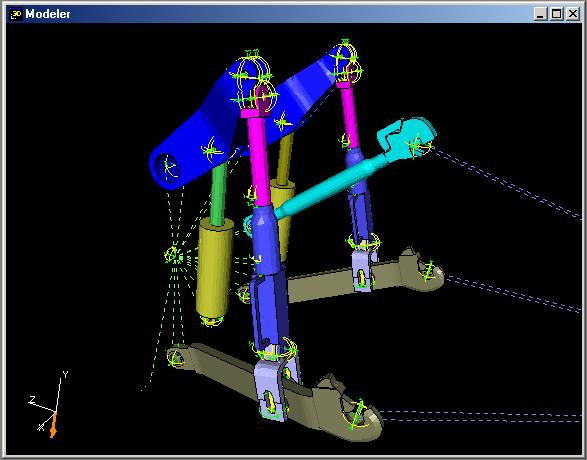
\includegraphics[width=0.93\textwidth]{Figures/3-Modeler}
\end{center}


\SubSection{Modeling tool bars}{modeling-tool-bars}

In Fedem, there are three major tasks performed by the user:
1) creating the mechanism and control system;
2) setting up and starting the analysis; and
3) setting up and viewing the results.
Each task has a different set of associated commands.
The modeling tools used to create and edit models are covered by the
\textbf{Mechanism Creation} tool bar and the \textbf{Mechanism Tools} tool bar.

\SubSubSection{Mechanism Creation tool bar}{mechanism-creation-tool-bar}

The \textbf{Mechanism Creation} tool bar (shown below) contains the mechanical
elements used to build Fedem mechanisms (see
\refSection{creating-mechanism-elements}{Creating creating mechanism elements}
for instructions on using these commands, and
\refChapter{mechanism-elements}{Mechanism Elements}
for a detailed description of each element).

\begin{center}
  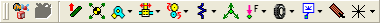
\includegraphics[height=1.5\baselineskip]{Figures/3-MechCreateToolbar}
\end{center}

\Note{An arrow ($\blacktriangledown$) beside a button indicates that
  more options can be accessed by clicking and holding down the button.}

\subsubsection {Mechanism Tools tool bar}

The \textbf{Mechanism Tools} tool bar (shown below) consists of modeling tools.
Each of these commands is described in the following sections.

\begin{center}
  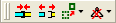
\includegraphics[height=1.5\baselineskip]{Figures/3-MechToolsToolbar}
\end{center}


%%%%%%%%%%%%%%%%%%%%%%%%%%%%%%%%%%%%%%%%%%%%%%%%%%%%%%%%%%%%%%%%%%%%%%%%%%%%%%%%
\Section{Mechanism modeling tools}{mechanism-modeling-tools}

To help you position items with greater accuracy and to simplify the modeling
process, Fedem provides some helpful modeling tools, including a reference
plane, an interactive point locator, point markers, and movability constraints.


\SubSection{Reference Plane}{reference-plane}

The Reference Plane is the shaded area in the center of the {\sl Modeler} view.
It serves both as a visual reference, and as a representation of the ground.

You can move it around, change its color and size, or turn it off so that it is
not visible in the {\sl Modeler} view.

To disable, enable or change the appearance of the Reference Plane, see
\refSection{general-appearance}{General Appearance} and
\refSection{item-appearance}{Item Appearance}.

\subsubsection{Changing the size}

To change the size of the Reference Plane, select the Reference Plane in the
{\sl Modeler} view (or Model Manager {\sl Objects} list), then edit its
{\sl Height} and {\sl Width} fields in the Property Editor panel (shown below).
Remember to press \textbf{Enter} after typing the values to apply the changes.

\noindent
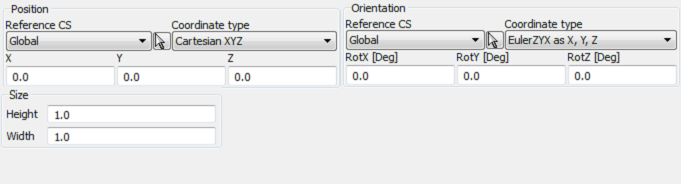
\includegraphics[width=\textwidth]{\ReferenceImg/prp/prp-reference-plane-1}

\subsubsection{Moving}

The Reference Plane is moved by editing the {\sl Position} and {\sl Orientation}
fields in the Property Editor panel.
See \refSection{origin-property}{Origin property}
for a detailed description of these data fields.

It is also possible to move the Reference Plane by aligning it to a specified
coordinate system in your model.
To do so, use the \textbf{Align CS} or \textbf{Align rotation} commands.
See \refSection{align-cs-and-rotations}{Align CS and rotations}.


\SubSection{Interactive Odometer and 3D Point Marker}{interactive-odometer}

\noindent
\begin{minipage}{0.77\textwidth}
  \raggedright
  Many Fedem commands require you to select a point in your model.
  To help you locate specific points, Fedem provides the Interactive Odometer
  and the 3D Point Marker (shown at right).
  These are displayed in the {\sl Modeler} view each time you select a point.
  The odometer shows the coordinates of the selected point, and the
  marker shows the location of the point in the {\sl Modeler} view.
\end{minipage}% <--- the % is needed here to kill off spurious spacing
\hfill\begin{minipage}{0.2\textwidth}
  \center
  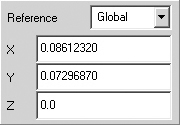
\includegraphics[width=\textwidth]{Figures/3-odometer} \\[2mm]
  
\includegraphics[width=0.25\textwidth]{Figures/3d_point_marker}
\end{minipage}

When using the \textbf{Smart Move} command to move or rotate parts and other
mechanism elements (see \refSection{moving-mechanism-elements}
{Moving mechanism elements}), the Interactive Odometer allows you to edit the
selected point or enter a new 3D point using global or local coordinates.
The local coordinate system used is the coordinate system of the item you
selected when the point was picked.

\Tip{You can use the Interactive Odometer with the \textbf{Smart Move} command
  to place a mechanism element (part, joint, triad, etc.) at any point in space.
  The object can then be used as a reference when moving other objects.}

To edit a point or enter a new point using the Interactive Odometer,
complete the following steps:

\begin{enumerate}
\item
  Select a point in the {\sl Modeler} view. The coordinates of the point
  (given in the local coordinate system for the selected element)
  are displayed in the Interactive Odometer, and the 3D Point Marker
  shows the location of the point selected.
\item
  Select {\sl Local} or {\sl Global} coordinates from the {\sl Reference}
  pull-down menu.
\item
  Type new values for the $X$-, $Y$- and $Z$-coordinates in the Interactive
  Odometer, and press the \textbf{Enter} key after editing the values.
  The 3D Point Marker is updated to show the new position.
\item
  When you are satisfied with the new location, press \textbf{Done} to confirm
  the selected point.
\end{enumerate}


\SubSection{Stickers}{stickers}

Stickers are movability constraints that are applied automatically when moving
mechanism objects with the \textbf{Smart Move} command
(see \refSection{moving-mechanism-elements}{Moving mechanism elements}).
Stickers can also be applied manually
(see \protect\hyperlink{manually-applying-stickers}
{\sl"Manually applying stickers"} below).
Each sticker applies the same constraint as a ball joint; in other words,
it constrains all translational motion.

\begin{wrapfigure}{r}{0.2\textwidth}
  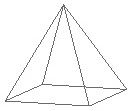
\includegraphics[width=0.2\textwidth]{Figures/sticker}
\end{wrapfigure}

Stickers are displayed in the {\sl Modeler} view as small pyramids
(shown at right). The tip of the pyramid is located at the constrained point.

When using \textbf{Smart Move}, the motion allowed, or movability, for a
selected object or group depends on the number and location of applied stickers.
Each move using \textbf{Smart Move} automatically applies an additional sticker.
Therefore, three successive moves of an initially free object (without stickers)
first results in a translation, then in rotation about a point, and lastly
rotation about the remaining axis. The object is then locked in place.
(See also \refSubSection{movability}{Movability}{smart-move}.)

\Important{Stickers function as modeling aids only.
  They are not considered part of the mechanism model,
  and therefore do not influence the mechanism motion during simulation.}

\SubSubSection{Manually applying stickers}{manually-applying-stickers}

Stickers are created automatically when using \textbf{Smart Move}, but you can
also create them manually when you need a certain type of movability.
To rotate about a point in space, apply one sticker at the rotation center.
To rotate about an axis, apply two stickers somewhere along the rotation axis.
Stickers are applied to Triads and Parts and can be positioned at any point in
space. They are not restricted to the geometry of visualization or the nodal
points of a part. To create a sticker, perform the following steps:

\IconText{sticker}{\vspace*{2mm}
  \begin{enumerate}
    \setlength\itemsep{1mm}
  \item
    Click the \textbf{Sticker} button on the \textbf{Mechanism Tools} tool bar.
    The Guide panel prompts you to select an application point for the sticker
    on an object.
  \item
    Place the cursor over the point on the object you want and press the left
    mouse button. The selection snaps to the nearest node (or point)
    on the object.
  \item If necessary,
    edit the position using the Interactive Odometer as described in
    \refSection{interactive-odometer}{Interactive Odometer and 3D Point Marker}.
  \item
    Confirm the point by clicking \textbf{Done}. The sticker is created, and
    the sticker symbol appears in the {\sl Modeler} view at the selected point.
\end{enumerate}}

\subsubsection{Deleting stickers}

You can delete stickers individually or all in a single operation.

\vskip19mm
\IconText{delete}{\vspace*{-18mm}
  \begin{itemize}
    \setlength\itemsep{1mm}
  \item To delete a single sticker, complete the following steps:
    \begin{enumerate}
      \setlength\itemsep{1mm}
    \item Select the sticker you want to delete in the {\sl Modeler} view or
      from the Model Manager {\sl Objects} list.
      The sticker symbol in the {\sl Modeler} view turns red when selected.
    \item Click the \textbf{Delete} button on the \textbf{Standard} tool bar
      or use the \textbf{Delete} key. The sticker is removed from the model.
    \end{enumerate}
  \end{itemize}}

\vskip-3mm
\IconText{deleteAllStickers}{\vspace*{1mm}
  \begin{itemize}
  \item To delete all the stickers applied to your model,
    click the \textbf{Delete All Stickers} button on the
    \textbf{Mechanism Tools} tool bar on the \textbf{Mechanism} menu.
  \end{itemize}}

\Note{You may have to click and hold down the \textbf{Sticker} button
  on the \textbf{Mechanism Tools} tool bar to access the
  \textbf{Delete All Stickers} command.}

\Warning{ There is no undo option after deleting all stickers.
  To replace them in your model, you must recreate each of them individually.}


%%%%%%%%%%%%%%%%%%%%%%%%%%%%%%%%%%%%%%%%%%%%%%%%%%%%%%%%%%%%%%%%%%%%%%%%%%%%%%%%
\Section{Creating mechanism elements}{creating-mechanism-elements}

Objects such as Spring/Damper characteristics, Functions, Frictions, Beam-
and material properties, which all do not need to be positioned are created
in the Model Manager {\sl Objects} list. Right-click an empty space in the
Model Manager panel and select \textbf{Create} to access the full list of
elements that can be created using the shortcut menu.

\Tip{It is also possible to create non-positioned mechanism objects by copying
  existing ones. This is useful if you need a property object (Function,
  Friction, Beam property, etc), which is nearly identical to other existing
  property objects in the model.
  To copy objects, select them in the Model Manager {\rm Objects} list,
  and then select \textbf{Copy Object} from the right-click menu,
  or from the \textbf{Edit} menu.}

All mechanism elements that need to be positioned in the Fedem model
are created by a different method. Normally,
you first need to select the position(s) needed to place the new element.
Then you sometimes need to orient the element properly,
and then you finally have to attach it. See
\refSection{moving-mechanism-elements}{Moving mechanism elements} and
\refSection{attaching-and-detaching-elements}{Attaching and detaching elements}.

The only exceptions to this are the parts and beams which are created
completely differently. Please have a look at
\refSection{creating-parts-by-file-import}{Creating parts by file import},
\refSection{creating-parts-from-hard-points}{Creating parts from hard points}
and \refSection{creating-beams}{Creating beams}.

To create a positioned mechanism element (except for parts and beams),
complete the following steps:

\begin{enumerate}
\item
  Click the button for the item on the \textbf{Mechanism Creation} tool bar
  (see \refSubSection{mechanism-creation-tool-bar}{Mechanism Creation tool bar}
  {modeling-tool-bars}).
\item
  Follow the instructions in the Guide panel while selecting one or more
  positions or related objects in the {\sl Modeler} view.
  Positions can also be entered by using the Interactive Odometer (see
  \refSection{interactive-odometer}{Interactive Odometer and 3D Point Marker}).
\item
  When you are satisfied with a selection, click \textbf{Done} to confirm.
  When all positions/selections are completed, the element is created using the
  selected position(s). A sticker is normally applied to the new object
  automatically to make it easy to rotate using \textbf{Smart Move}.
\item
  You can then use \textbf{Smart Move} or some other means to adjust the
  object's orientation (see \refSection{stickers}{Stickers} and
  \refSection{moving-mechanism-elements}{Moving mechanism elements}).
\item
  As the last operation you need to attach the object to a part or a
  beam using the \textbf{Attach} command. See
  \refSection{attaching-and-detaching-elements}
             {Attaching and detaching elements}.
\end{enumerate}

\Tip{To edit the properties of a new mechanism element, select the item in
  the {\rm Modeler} view or Model Manager {\rm Objects} list.
  The properties of the item are then displayed in the Property Editor panel.}


\SubSection{Selecting position and orientation}
           {selecting-position-and-orientation}

When creating mechanism elements, you are asked to select their position.
Revolute joints, Free joints, Loads and master triads of Cam joints
will be created with a default orientation as well.

As you select a point, Fedem will snap to geometric features and also extract a
default orientation if necessary, by different rules depending on what type of
object you hit.

\subsubsection{Snapping and default orientation on FE Parts}

When picking an FE surface the default orientation is set to be perpendicular to
that surface and the position snaps to the closest node.
If the exact position of the mouse is on an FE mesh line, however,
the default orientation is aligned with the direction of that line.
It is the exact mouse position that decides whether you hit a line or a surface,
even when the 3D Point Marker snaps to the same node.

\subsubsection{Snapping and default orientation on CAD Parts}

\noindent
\begin{minipage}{0.75\textwidth}
  \raggedright
  If the mouse position is on a CAD part, the geometry of the face or edge
  is used to extract a default orientation and a snap point.
  If the face or edge in question is a revolved geometry,
  the options shown to the right pop up in the Guide panel.
  These options allow you to control how the snap point and
  the default orientation is extracted from the geometry.
\end{minipage}% <--- the % is needed here to kill off spurious spacing
\begin{minipage}{0.25\textwidth}
  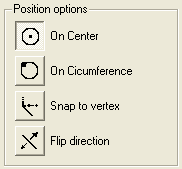
\includegraphics[width=\textwidth]{Figures/3-SnapPanel}
\end{minipage}

You can here choose whether the point shall snap to the center axis of the
revolved face ({\sl On Center}) with the default orientation along that axis,
or to the circumference of the revolved geometry ({\sl On Circumference})
with the default orientation perpendicular to the face.

The default orientation can be flipped to the opposite direction using
the {\sl Flip Direction} option.

The {\sl Snap To Vertex} option controls whether or not the selected point shall
snap to the closest vertex. In combination with {\sl On Circumference},
the point will snap to the closest vertex on the surface,
whereas with {\sl On Center} it will snap to the point on the center axis
which is closest to the vertex.

\clearpage

\subsubsection{Default direction notes}

\noindent
\begin{minipage}{0.7\textwidth}
  \raggedright
  The default direction is visualized as a yellow arrow (as shown to the right)
  starting from the selected point.
  The following object types utilize the default direction arrow:

  \begin{itemize}
  \item{\sl Force and Torque} -- the attack direction.
  \item{\sl Revolute joint} -- the axis of rotation.
  \item{\sl Cam joint master triads} -- the $X$-direction (up)
    of the master triads are aligned with the default direction.
  \item{\sl Free joint} -- $Z$-axis of the master.
  \end{itemize}
\end{minipage}% <--- the % is needed here to kill off spurious spacing
\hfill\begin{minipage}{0.22\textwidth}
  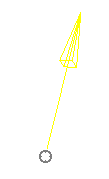
\includegraphics[width=\textwidth]{Figures/3-Default-createDirection-sec-3-4}
\end{minipage}


%%%%%%%%%%%%%%%%%%%%%%%%%%%%%%%%%%%%%%%%%%%%%%%%%%%%%%%%%%%%%%%%%%%%%%%%%%%%%%%%
\Section{Moving mechanism elements}{moving-mechanism-elements}

Fedem provides several commands and tools for moving parts of your model:
\textbf{Smart Move}, \textbf{Align CS}, \textbf{Align rotations} and
\textbf{Move To Center} are all useful commands, while the {\sl Origin} tab
of the Property Editor panel, that several mechanism objects share, can be used
to access the position and orientation of a single component directly.


\SubSection{Smart Move}{smart-move}

The \textbf{Smart Move} command is an integral part of 3D modeling in Fedem.
It is a sophisticated way to position and orient mechanism entities,
such as parts, triads, joints, springs, dampers, and so on.
This command enables you to move or orient an object or a group of objects
according to the selection's current movability (see below).
During a \textbf{Smart Move}, a movability constraint (called a Sticker)
is automatically created (see \refSection{stickers}{Stickers}).

\SubSubSection{Movability}{movability}

The movability of an object or a group of objects is determined by examining not
only the stickers that are applied to the selection, but also the joints between
the selected object/group and other objects.
Each joint or sticker that constrains the group reduces its movability.
The following symbols represent the six types of motion allowed when using
the \textbf{Smart Move} command:

\def\RightFigure#1#2{\noindent
  \begin{minipage}{0.65\textwidth}
    \raggedright#2
  \end{minipage}% <--- the % is needed here to kill off spurious spacing
  \hfill\begin{minipage}{0.25\textwidth}
    \includegraphics[width=0.8\textwidth]{Figures/#1}
  \end{minipage}}

\RightFigure{SmartMoveFree}{{\sl Free} --
  when an object without stickers or attached joints is moved with
  the \textbf{Smart Move} command, it can move in translation in any direction.
  The symbol for free movement is depicted in the {\sl Modeler} view
  as shown to the right.}

\RightFigure{SmartMoveBall}{{\sl Ball} --
  when one sticker or one ball joint has been applied to a mechanism entity,
  it can rotate about the point at which the sticker/joint is applied.
  The symbol for ball movement is depicted in the {\sl Modeler} view
  as shown to the right.}

\RightFigure{SmartMoveRevolve}{{\sl Revolving} --
  when two stickers (or one ball joint and one sticker or two ball joints)
  have been applied to a selection of mechanism elements, the stickers/joints
  act together as a revolute joint with the axis defined by the line between
  the two stickers/joints.
  The symbol for revolving motion is depicted in the {\sl Modeler} view
  as shown to the right.}

\RightFigure{SmartMoveExtra1}{{\sl Cylindric} --
  when a selection of mechanism elements is constrained by a cylindrical joint,
  the selection can be translated along and rotated about the joint axis.
  The symbol for cylindrical motion is deprecated in the {\sl Modeler} view
  as shown to he right.}

\vskip\parskip
\RightFigure{SmartMoveExtra2}{{\sl Prismatic} --
  when a selection of mechanism elements are constrained by a prismatic joint,
  the selection can be translated along the joint axis.
  The symbol for prismatic motion is depicted in the {\sl Modeler} view
  as shown to the right.}

\vskip\parskip
\RightFigure{SmartMoveRigid}{{\sl Rigid} --
  when three stickers or ball joints (not located on a straight line)
  are applied to a selection of mechanism elements, the selection is fully
  fully constrained and cannot be moved with the \textbf{Smart Move} command.
  The symbol for rigidity (no movement allowed) is depicted in
  the {\sl Modeler} view as shown to the right.}

\subsubsection{Performing a Smart Move}

\vskip8mm\hskip\parindent
\IconText{smartMove}{\vspace*{-10mm}
  To move an object or group of objects using the \textbf{Smart Move} command,
  complete the following steps:}

\vspace*{-9.5mm}
\begin{enumerate}
\item
  Click the \textbf{Smart Move} button from the {\sl Mechanism Tools} tool bar.
  The Guide panel prompts you to select objects to move.

\item
  To select an object and indicate the from-point, place the cursor over a point
  on the object and press the left mouse button.
  The selection snaps to the nearest node or point on the object.
  This point becomes the from-point and a symbol is shown that depicts
  the movability of the current selection.

  \EnumTip{Several objects can be selected by pressing and holding the
    \textbf{Ctrl} key while selecting objects. To change the last selected
    object only, release the \textbf{Ctrl} key and select until you hit the
    right object. To remove several of the last selected objects from the
    selection, release the \textbf{Ctrl} key, and press the left mouse
    button on some empty space in the. {\rm Modeler} view until all the
    objects in question is deselected.}

  \EnumTip{You can also type in a discrete point or edit the point using the
    Interactive Odometer (see \refSection{interactive-odometer}
    {Interactive Odometer and 3D Point Marker}).}

\item
  When you are satisfied with the object and the from-point selected,
  press \textbf{Done} to confirm it. The Guide panel then prompts for
  you to select a to-point.

\item
  Select the to-point in the same way you selected the from-point, and if
  necessary, edit it using the Interactive Odometer to specify a discrete point.

\item
  When you are satisfied with the to-point, press \textbf{Done} to confirm it.
  The move operation is animated in the {\sl Modeler} view.
\end{enumerate}


\SubSection{Align CS and rotations}{align-cs-and-rotations}

Two commands are provided to align one or several objects to an existing
coordinate system in your model:

\IconText{alignCS}{
  The \textbf{Align CS} command will both translate and rotate the selected
  objects to match their coordinate systems (CS) with a selected object.}

\IconText{alignRotations}{
  The \textbf{Align rotations} command only rotates the selected objects.}

\subsubsection{Performing an Align command}

To move an object or group of objects using one of the align commands,
complete the following steps:

\begin{enumerate}
\item
  Click the appropriate align button in the \textbf{Mechanism Tools} tool bar.
  They are located under the \textbf{Smart Move} icon.

\item
  Select the objects to move by picking them in the {\sl Modeler} view.
  Press \textbf{Done} to confirm the selection.

  \EnumTip{Several objects can be selected by pressing and holding the
    \textbf{Ctrl} key while selecting objects. To change the last selected
    object only, release the \textbf{Ctrl} key and select until you hit the
    right object. To remove several of the last selected objects from the
    selection, release the \textbf{Ctrl} key, and press the left mouse
    button on some empty space in the {\rm Modeler} view until all the
    objects in question are deselected.}

\item
  Select the coordinate system to align to by picking an object that is defined
  in that coordinate system.
  The selected coordinate system will be displayed in red.
  Press \textbf{Done} to confirm the selection and execute the move.

  \EnumTip{The \textbf{Align} commands can be used to align objects to local FE
    coordinate systems, if present. The visibility of local coordinate systems
    can be toggled using the General Appearance dialog box.
    See \refSection{general-appearance}{General Appearance}.}
\end{enumerate}


\SubSection{Move To Center}{move-to-center}

This is a useful tool if you want to position an object at the center of some
geometry. The object will move to the center of a circle you define,
or somewhere along its axis. The new orientation of the object aligns with
the circle. The $X$-axis is defined by the center and the first point defining
the circle, the $Z$-axis is perpendicular to the circle.

\subsubsection{Performing a Move To Center}

\vskip8mm\hskip\parindent
\IconText{moveToCenter}{\vspace*{-10mm}
  To move an object or group of objects using the \textbf{Move To Center}
  command, complete the following steps:}

\vspace*{-10mm}
\begin{enumerate}
\item
  Click the \textbf{Move To Center} button in the \textbf{Mechanism Tools}
  tool bar. It is located under the \textbf{Smart Move} icon.

\item
  Select the objects to move by picking them in the model view.
  Press to confirm the selection.

  \EnumTip{Several objects can be selected by pressing and holding the
    \textbf{Ctrl} key while selecting objects. To change the last selected
    object only, release the \textbf{Ctrl} key and select until you hit the
    right object. To remove several of the last selected objects from the
    selection, release the \textbf{Ctrl} key, and press the left mouse
    button on some empty space in the {\rm Modeler} view until all the
    objects in question are deselected.}

\item
  Select three points of the perimeter defining a circle.
  Confirm each point by pressing \textbf{Done}.
  After setting the third point the defined circle will appear in the
  {\sl Modeler} view.

\item
  You may now select a point to place your objects along the circles axis, or
  press \textbf{Done} once more to move the objects to the center of the circle.
\end{enumerate}


\SubSection{Origin property}{origin-property}

Triads, parts, and point-to-point joints have a property tab called
{\sl Origin} (shown below). This property tab is used to display and edit the
position and orientation of the mechanism element in question.
The sensitivity of the fields will reflect whether the selected object is
allowed to move considering its attachments, etc., without corrupting the model.

\noindent
\begin{picture}(340,85)
  \put(0,0){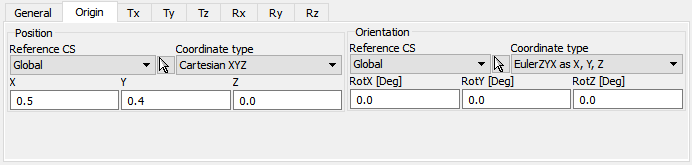
\includegraphics[width=\textwidth]{\ReferenceImg/prp/triad-2}}
  \put( 25,60){\Bullet{1}}
  \put(205,60){\Bullet{2}}
  \put( 36,44){\Bullet{3}}
  \put(206,44){\Bullet{3}}
  \put(130,44){\Bullet{4}}
  \put(305,44){\Bullet{5}}
\end{picture}

\begin{bulletlist}
\item{\sl Position} --
  displays the data for the translational part of the position.
\item{\sl Orientation} --
  displays the data for the rotational part of the position.
\item{\sl Reference CS} --
  The translation and rotation can both be displayed and edited
  in any coordinate system in the model.
  These pull-down menus allows the reference coordinate systems to be selected.
  They can also be selected by picking in the {\sl Modeler} view or selected
  from the {\sl Objects} list of the Model Manager panel.
  To do so, you must first click the arrow button next to the pull-down menu.
  The Guide panel tells you to select a reference CS.
  Select a triad, a beam or a part, when satisfied, press \textbf{Done}.
\item{\sl Coordinate type} --
  This menu controls whether to display the translation in Cartesian coordinates
  or cylindrical coordinates. The cylindrical coordinates can use either $X$,
  $Y$ or $Z$ as the rotational axis.
\item{\sl Coordinate type} --
  This menu controls how to edit and display the orientation.
  The Orientations input type options are:
  \begin{itemize}
  \subitem
  Angles about the $X$-, $Y$- and $Z$-axis in degrees.
  The parameterization used is the one called Euler-ZYX, which means a rotation
  about the $Z$-axis of the reference CS first, next the $Y$-axis, and finally
  the $X$-axis. (This can also be understood as a rotation about the axes of the
  with-rotated (or local) $X$-axis first, then local $Y$ and finally local $Z$.)
  \subitem
  A point on the $X$-axis, and a point in the $XY$-plane.
  The $X$- and $Y$-direction is then computed from the given point and
  the translation of the object.
  \subitem
  A point on the $Z$-axis, and a point in the $XZ$-plane.
  \subitem
  An $X$-direction vector and a vector in the $XY$-plane.
  In this mode, the $X$- and $Y$-vectors form a $3\times3$ rotation matrix
  that can be used directly.
\end{itemize}
\end{bulletlist}

\Note{The center of the applied rotations are always the origin of
  the coordinate system in question (the position controlled by the
  Position options) and not at the origin of the selected reference CS.}

\subsubsection{Visualization}

\begin{minipage}{0.4\textwidth}
  \raggedright
  The sizes displayed in the {\sl Position} frame are visualized, along with
  with the reference CS for the orientation, whenever the {\sl Origin} property
  is visible. The visual appearance of this visualization is shown to the right.
\end{minipage}% <--- the % is needed here to kill off spurious spacing
\hfill\begin{minipage}{0.5\textwidth}
  \begin{picture}(150,95)
    \put(0,0){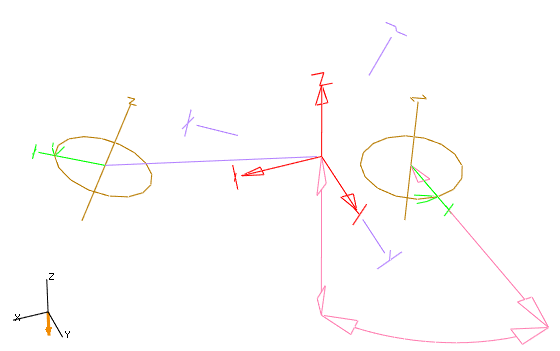
\includegraphics[width=\textwidth]{Figures/3-OriginTabVisualization_1}}
    \put( 84,61){\Bullet{1}}
    \put(145, 8){\Bullet{2}}
    \put(130,55){\Bullet{3}}
    \put( 30,35){\Bullet{4}}
    \put(102,91){\Bullet{5}}
  \end{picture}
\end{minipage}

\begin{bulletlist}
\item{\sl The object to move (red)} --
  In this example; a Triad.
\item{\sl Position arrows (pink)} --
  Shows the various dimensions corresponding to the selected
  {\sl Coordinate Type as arrows} extending from the reference CS
  for the position.
\item{\sl Reference CS for the position}.
\item{\sl Reference CS for the Orientation} --
  The reference CS for the Orientation is shown by a purple line
  from the object to move to the reference CS.
\item{\sl Orientation Reference direction} --
  The reference directions for the orientation are shown as purple lines
  and letters indicating the orientation of the reference superimposed
  on the position of the object.
\end{bulletlist}


%%%%%%%%%%%%%%%%%%%%%%%%%%%%%%%%%%%%%%%%%%%%%%%%%%%%%%%%%%%%%%%%%%%%%%%%%%%%%%%%
\Section{Attaching and detaching elements}{attaching-and-detaching-elements}

Nearly all mechanism elements created in Fedem needs to be attached to a part or
a beam (or two parts or beams). The concept of attaching is to connect the joint
constraints, loads, etc., to the parts/beams they affect.

When attaching, two things happen: Firstly a triad in the element in question is
noted to be connected to the part/beam (see also \refSection{triads}{Triads}).
All the constraints, loads, etc., that the element introduces will then be
working on that particular part or beam.
Secondly, if attaching to an FE part, the triad is connected to the FE mesh
of the part, either by direct association with an existing FE node in the part,
or by using a {\sl Surface connector} to distribute the forces in some way.

When an element has been attached, it can generally not be moved relatively to
the object it is attached to. The \textbf{Detach} command is used to
disconnect a mechanism element from the part or beam it is attached to,
making it possible to move it around again.

\SubSection{Using the Attach command}{using-the-attach-command}

The \textbf{Attach} command can be used when an element is to be connected to
ground, to a beam, to a {\sl Generic Part}, or to an {\sl FE part}
with an existing FE node at the attach point.
To attach a mechanism element using the \textbf{Attach} command,
complete the following steps:

\vskip\parskip
\IconText{attach}{\vskip-5mm
  \begin{enumerate}
    \setlength\itemsep{1pt}
  \item
    Click the \textbf{Attach} button on the \textbf{Mechanism Tools} tool bar
    (or select from the \textbf{Mechanism} menu). The Guide panel then prompts
    you to select a mechanism element to attach to the model.
  \item
    Select the element in the {\sl Modeler} view.
  \item
    When you have made your selection, press \textbf{Done} to confirm it.
    The Guide panel then prompts you to select a part (or beam) onto which
    to attach the object.
  \item
    Select a part, a beam, or the reference plane in the {\sl Modeler} view
    and press \textbf{Done} to confirm the selection.
    The object becomes attached to the selected part or beam,
    or to the ground if the reference plane was selected.
  \end{enumerate}}

\Tip{Watch the Output List view for messages during the attachment process.
  If an attachment cannot be completed, an error message is displayed here.}

\Note{Triads in axial springs, dampers, and loads are automatically attached
  when created, because the orientation of such triads is not important.}

\subsubsection{Attaching joints}

Joints consists of one slave triad and one or more master triads. The slave
triad is normally attached to one FE model, and the master triad(s) to another.
This is done by attaching one part of the joint first, and then the other one.
See \refSection{joints}{Joints} for more information about master- and slave
triads in joints. When attaching by selecting the joints directly,
Fedem automatically selects which triad (master or slave) to attach first.
In most cases, the slave is attached first.

To control whether a joint's slave or master is attached to a specific node,
select only the part of the joint symbol that represents that particular triad
when selecting the object to attach during the \textbf{Attach} command.
See \refSection{joints}{Joints} for more information about joint symbols.

\Tip{To attach multiple {\sl joints} to a single FE node,
  you must align the master triads of the joints.
  You can then attach the master triads of each joint to the FE node. The two
  master triads will then be merged into one triad shared by the two joints.}


\SubSection{Surface Connectors}{surface-connectors}

\hskip\parindent
\IconText{spider}{
  The \textbf{Surface connector} commands are used to attach mechanism elements
  to FE parts at positions without existing FE nodes (e.g., at center of holes),
  or in such a way that the Surface connector distributes the forces from the
  joint, load, etc., onto some area on the FE model.}

Surface connectors connect a triad to an FE model using two different
connection types, {\sl Rigid Surface} or {\sl Flexible Surface}.

\vskip2\parskip
\IconText{spiderGen}{\textbf{Flexible surface}}
\vskip-5mm
\RightFigure{3-SpiderFlexible}{
  The Flexible surface connector acts as a force distributor.
  It does not introduce stiffness or constraints between the FE nodes
  it connects to, but distributes the forces from the triad onto the FE model.
  The Flexible surface connector is visualized with dotted lines,
  as shown to the right.}

Each nodal DOF gets an equal share of the translational forces in the triad.
The moments acting on the triad, and the moment created by the translational
forces about the geometrical center of the nodes, is balanced by an additional
force in each node, weighted by the nodes distance from the geometrical center
of the nodes in the Surface connector. In the case where the nodes also have
rotational DOFs (shell nodes), those rotational DOFs also gets an equal share
of the moment.

\vskip2\parskip
\IconText{spiderGeom}{\textbf{Rigid surface}}
\vskip-5mm
\RightFigure{3-SpiderRidig}{
  The rigid surface connector is a rigid connection between the triad and
  all the FE nodes it connects. That means that all the FE nodes connected
  with the surface connector becomes one rigid block.
  The rigid surface connector is visualized with dashed lines.}


\SubSection{Surface connector commands}{surface-connector-commands}

There are two ways of creating a Surface connector:
\textbf{By selecting nodes} or \textbf{By cylinder surface}.
These commands can either create a new connected triad at a user-defined
position, or connect an existing triad to the FE mesh, in somewhat the same
manner as the \textbf{Attach} command.

\subsubsection{By selecting nodes}

\IconsText{spiderGenRBE2}{spiderGenRBE3}{
  These commands are used to select arbitrary nodes or areas of nodes
  to use for the Surface connector.
  To create a Surface connector by selecting nodes,
  complete the following steps:}

\begin{enumerate}
\item
  Select either the rigid or flexible version of the command.
  \begin{center}
    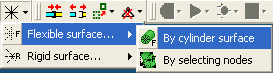
\includegraphics[width=0.4\textwidth]{Figures/3-SpiderByCylinder}
  \end{center}

\item
  First you have the option to either select an existing triad, which
  might be embedded in a mechanism element, or to select a position
  where you want a new triad to be created.
  If you pick a triad, that triad will become selected and will be
  attached through the surface connector. If you pick something else, the
  snap-point will be used as the position for a new triad.
  If you get it wrong, try again until you have selected what you want,
  then accept by pressing \textbf{Done}.

\item
  Now you need to select all the FE nodes to be connected to the triad.
  You can add single nodes to the selection by picking, or all visible surface
  nodes within a rectangle by dragging a window.
  If you press and hold the \textbf{Ctrl} key, picked or window-selected nodes
  will be removed from the selection instead of being added.
  When finished, press \textbf{Done}.
\end{enumerate}

\subsubsection{By cylinder surface}

\IconsText{spiderGeomRBE2}{spiderGeomRBE3}{
  These commands create a Surface connector from nodes on the surface
  of a cylinder volume. It is convenient to use them to attach a mechanism
  element to the inside of a hole, a circular edge, etc.
  The command is also able to place a new triad along the axis of the cylinder,
  making it easy to get the hard-points.
  This triad can then be used for further modeling.}

The cylinder is defined by a 3-point circle,
together with points on each end of the cylinder.
To create a Surface connector by cylinder surface, complete the following steps:

\begin{enumerate}
\item
  Select either the rigid or flexible version of the command.
  \begin{center}
    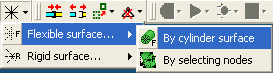
\includegraphics[width=0.4\textwidth]{Figures/3-SpiderByCylinder}
  \end{center}

\item
  You have the option to select either an existing triad that will be attached
  by the Surface connector, or a position where a new triad will be created.
  If you want the command to create a triad along the cylinder axis,
  start by selecting the tree nodes that define the circle.
  If you pick a triad, that triad will be attached using the surface connector.
  If you pick an FE node, the node will be used as the first of three nodes that
  defines the cylinder circle. If you pick something else,
  the snap-point will be used as the position for a new triad.
  If you get it wrong, try again until you have selected what you want,
  then accept by pressing \textbf{Done}.

\item
  Then select the rest of the tree points defining the cylinder circle,
  accepting each node by pressing \textbf{Done}.
  A cylinder/circle visualization will show the resulting cylinder
  as you select the last node.

\item
  When the cylinder circle is defined, you can now or after any of the following
  steps press \textbf{Done} to complete the command using the definition of the
  cylinder that is shown.
  The optionally new triad will then be created in the center of the circle,
  if you did not define a position for it in the start of the command.

\item
  The next steps is to select the start and end of the cylinder.
  Do this by selecting an FE node for the start, and one for the end.
  Accept each of them by pressing \textbf{Done}.

\item
  Finally the position of the optionally new triad along the cylinder axis
  can be selected. Press \textbf{Done} to accept.
\end{enumerate}

When the command is completed, Fedem selects all the nodes from the FE model in
question that is on the surface of the cylinder volume defined. These nodes
are now connected to the new or existing triad by the Surface connector.

\subsubsection{Deleting or redefining Surface connectors}

A surface connector is actually an attribute of the Triad it connects.
This means that if the triad is detached, the connector is deleted.

If a connector needs to be edited or changed, simply use one of the surface
connector commands to redefine it. Invoke the command, and select the triad with
the mis-defined connector at the start of the command sequence.


\SubSection{Attachment rules and restrictions}
           {attachment-rules-and-restrictions}

There are several restrictions and rules that apply to the connections between
FE models and triads. These restrictions do not apply when attaching triads to
{\sl Generic Parts} or {\sl Beams.}

\begin{itemize}
\item
  The triad and the FE node must be within the distance set by the modeling
  tolerance (see \refSection{modeling-tolerance}{Modeling tolerance}).
  If several nodes exist within the modeling tolerance,
  the one closest to the triad will be selected.
\item
  Slave triads can not be attached to ground.
  Joints must be attached to the ground by their master triads.
\item
  Two or more slave triads can not be attached to the same FE node.
\item
  Master triads or triads where the triad directions is referenced must
  be aligned before they can be attached to the same FE node.
\end{itemize}

\Note{When several elements are attached to the same node, the triads in those
  elements are merged into the triad already attached. This resulting triad is
  then shared by all the attached elements. (The redundant triads are removed.)}

\Note{When a triad is attached to a FE model at the position of a slave FE node,
  Fedem will automatically add a 6-DOF node, a spring and a mass element to the
  FE model at that point. The triad is then attached to the new 6-DOF node
  instead of the slave node to overcome limitations in the mathematical method.
  The spring stiffness and mass is set automatically by the FE part reducer to
  a very high stiffness, and a very low mass compared to the actual model in
  question. However, if the part is completely rigid
  (e.g., it consists of a single RGD element), the value $2\times10^{11}$
  is used for stiffness and no mass is added. See also
  the \FedemTGuide{Section A.10, "BUSH"} and {\sl Section A.12, "CMASS"}.}


\SubSection{Detaching}{detaching}

To detach mechanism elements from your model, complete the following steps:

\IconText{detach}{\vskip-5mm
  \begin{enumerate}
    \setlength\itemsep{1mm}
  \item
    Click the \textbf{Detach} button on the \textbf{Mechanism Tools} tool bar
    (or select from the \textbf{Mechanism} menu.
  \item
    Select the item(s) to detach (hold down the \textbf{Ctrl} key
    while selecting multiple items in the {\sl Modeler} view).
  \item
    Click \textbf{Done} to confirm your selection.
    The object(s) are detached from your model.
 \end{enumerate}}

\Note{When detaching a joint, both the master and slave triads are detached.
  If you want to detach only one of them, press the \textbf{Detach} button,
  then select the part of the joint symbol that represents either the master
  or the slave triad and press \textbf{Done}.}


\SubSection{Color of attached and unattached elements}
           {color-of-attached-and-unattached-elements}

The color of a mechanism element indicates whether or not it is attached
to the model. If the element's symbol is white (the default color), it
is not fully attached. A colored symbol indicates that an element is
attached.

\Tip{The colors for attached and unattached elements can be changed in the
  General Appearance dialog box
  (see \refSection{general-appearance}{General Appearance}).}


\SubSection{Invalid attachments}{invalid-attachments}

\begin{wrapfigure}{r}{0.3\textwidth}
  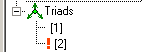
\includegraphics[width=0.3\textwidth]{Figures/3-AttachInvalidTriad}
\end{wrapfigure}

At some points Fedem may find that some Triads in your model does not correspond
to an underlying FE node even if it should have. Fedem will then warn you with
a dialog box, and mark all the invalidly attached triads with a red exclamation
mark in the Model Manager {\sl Objects} list.

The model will not be solvable as long as you have invalidly attached triads.
To resolve this you have several options:

\begin{itemize}
\item
  Use a surface connector to connect the triad to a set of existing FE nodes.
\item
  You can move the triads to the correct positions.
\item
  Update the FE mesh with nodes at the correct positions.
\item
  Turn the FE part into a Generic Part.
\item
  Delete the Triads.
\end{itemize}


%%%%%%%%%%%%%%%%%%%%%%%%%%%%%%%%%%%%%%%%%%%%%%%%%%%%%%%%%%%%%%%%%%%%%%%%%%%%%%%%
\Section{Deleting mechanism elements}{deleting-mechanism-elements}

Fedem uses the \textbf{Delete} command to remove mechanism elements from
a model. The \textbf{Delete} command can be used in two different ways;
in the {\sl Modeler} view or in the Model Manager panel.


\SubSection{Deleting in the Modeler view}{deleting-in-the-modeler-view}

To delete elements in the {\sl Modeler} view, complete the following steps:

\vskip14mm
\IconText{delete}{\vspace*{-13mm}
  \begin{enumerate}
    \setlength\itemsep{1mm}
  \item In the {\sl Modeler} view, select the element to be deleted,
    or hold down the \textbf{Ctrl} key and select multiple items.
    The selected items are highlighted in red.
  \item To remove the selected element(s) from the model,
    click the \textbf{Delete} button on the \textbf{Standard} tool bar
    or hit the \textbf{Delete} key.
  \end{enumerate}}

\Warning{There is no undo option after deleting objects.
  To replace mechanism elements after deleting them,
  you must recreate each one of them individually.}


\SubSection{Deleting in the Model Manager panel}{deleting-in-the-model-manager-panel}

To delete mechanism elements in the Model Manager panel,
complete the following steps:

\begin{enumerate} \setlength\itemsep{1em}
\item
  In the {\sl Objects} list, select the item to be deleted, or hold down the
  \textbf{Shift} or \textbf{Ctrl} key and select multiple items.
  The selected items are highlighted in red in the {\sl Modeler} view.

  \EnumTip{You can also click and drag the cursor to select multiple items
    for deletion.}

  \vspace*{-3mm}
\item
  To remove the element(s) from the model, right-click and select
  \textbf{Delete} from the shortcut menu (or hit the \textbf{Delete} key).
  The items are removed from both the model and the list at the same time.
\end{enumerate}

\Note{When deleting parts and beams, you have the option to retain triads that
  are attached to each deleted part/beam (except for joint triads -- they
  are always retained), to also delete those triads, or to cancel the
  \textbf{Delete} command. If no such triads exist for a selected part or
  beam, you must anyway confirm the deletion of the part/beam. This choice
  must be made for each part and beam in the selection. However, by
  selecting the \textbf{Yes to all}, \textbf{No to all} or \textbf{Ok to
  all} button, you automatically repeat the same choice for each part and
  beam in the current selection.}

\Note{If any of the objects you delete are referred to by a curve, you will be
  able to choose to either delete that specific curve definition, leave
  the curve definition intact while still deleting the object, or cancel
  deletion of the selected object.}

\Warning{If the deletion of a selected object also causes deletion of other
  objects connected to it, and any of these other objects also are referred
  to by a curve, you will be notified and can choose whether to delete that
  specific curve definition or not, too.
  However, you can not choose to cancel the delete operation at this stage.}


%%%%%%%%%%%%%%%%%%%%%%%%%%%%%%%%%%%%%%%%%%%%%%%%%%%%%%%%%%%%%%%%%%%%%%%%%%%%%%%%
\Section{Using file references in mechanism elements}
        {using-file-references-in-mechanism-elements}

\IconTextFirst{fileReference}{\vspace{-1mm}
  Some mechanism elements in Fedem need input from external files.
  For such elements the use of file references may be beneficial.
  The file reference replaces the file name in the element definition.
  As the contents of the file reference, the file it is referring to,
  is changed, so is the element input. Thus,
  if several mechanism elements receive input from the same file reference,
  and the contents of the file reference changes,
  so does the input of all elements using it.}

File references are created either by choosing \textbf{File reference...}
from the \textbf{Mechanism} menu, or by right-clicking an empty space in
the {\sl Objects} list of the Model Manager panel, choosing \textbf{Create}
and then \textbf{File reference...}.
Then select one or more files in the dialog box that appears.
One File reference object will be created for each file selected.

File references are set as input in mechanism elements by choosing the wanted
reference from the pull-down menu of the input file field.

\clearpage

%%%%%%%%%%%%%%%%%%%%%%%%%%%%%%%%%%%%%%%%%%%%%%%%%%%%%%%%%%%%%%%%%%%%%%%%%%%%%%%%
\Section{Model preferences}{model-preferences}

\begin{wrapfigure}[19]{r}{0.5\textwidth}
  \begin{picture}(155,225)
    \put(0,0){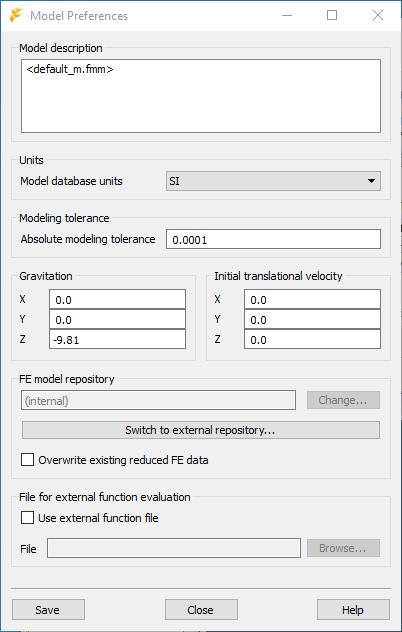
\includegraphics[width=0.45\textwidth]{\ReferenceImg/dlg-model-preferences}}
    \put(35,200){\Bullet{1}}
    \put(-8,168){\Bullet{2}}
    \put(-8,148){\Bullet{3}}
    \put(21,115){\Bullet{4}}
    \put(99,115){\Bullet{5}}
    \put(-8, 84){\Bullet{6}}
    \put(-8, 60){\Bullet{7}}
    \put(-8, 43){\Bullet{8}}
  \end{picture}
\end{wrapfigure}

In the Model Preferences dialog box you can adjust several global parameters
regarding the model.

\begin{bulletlist}
\item{\sl Model description} -- \newline
  This field lets you add notes \newline to your model file.
\item{\sl Units} --
  The consistent unit set to use.
  See \refSection{model-database-units}{Model database units}.
\item{\sl Modeling tolerance} -- The \newline
  maximum allowed distance \newline
  between the FE node and \newline its attached Triad. \newline
  See \refSection{modeling-tolerance}{Modeling tolerance}.
\item{\sl Gravitation} -- \newline
  The gravity vector direction and magnitude.
  See \refSection{gravitation}{Gravitation}.
\end{bulletlist}

\begin{bulletlist}
  \setcounter{enumi}{4}
\item{\sl Initial translational velocity} --
  The initial translational velocity of all triads in the model. See
  \refSection{initial-translational-velocity}{Initial translational velocity}.
\item{\sl FE model repository} --
  Switch between external and internal model repositories.
  You may also \textbf{Change} the external FE model repository. See
  \refSubSection{setting-the-fe-model-repository}
                {Setting the FE model repository}{using-fe-model-repositories}.
\item{\sl Overwrite existing reduced FE data} -- If enabled,
  any existing data in the FE model repository for an FE part that is reduced
  will be overwritten, instead of creating a new parallel sub-folder for it.
  Use this if your model consists of large FE parts that are reduced several
  times during modeling sessions, in order to save disk space.
\item{\sl File for external function evaluation} -- If enabled,
  you can browse for a file from which the
  \protect\hyperlink{external-function}{\sl External function} is in the model
  will take their values, instead of expecting them from an outside process.
  See \refSection{external-function-from-file}
  {External function values from file}.
\end{bulletlist}

\Note{Changes to the Model description notes will be saved also when closing
  the Model Preferences dialog box (using the \textbf{Close} button).
  Therefore, you may edit these notes at any time, also when you have results.}


\SubSection{Model database units}{model-database-units}

All modeling in Fedem is unit independent. However, some external interfaces
may require SI units in their calculations.

When modeling in other units than SI, you will then need to change the model
database units. Do this by selecting the model database units corresponding to
your model. The chosen units are then used to properly scale calculated data
before communicating with the external modules that require a specific unit set.

\Tip{You can add your own modeling units by editing the file \File{units.fcd}
  in any text editor. This file is located in the Fedem installation directory.}


\SubSection{Modeling tolerance}{modeling-tolerance}

The modeling tolerance is a tolerance that controls how strict Fedem enforces
that triads and their corresponding FE nodes are coincident.
This tolerance needs to be strict, because an offset will introduce an error
and inconsistence in the numerical model which might have serious impact on the
reliability of the results.

The seriousness is however depending on the size of the offset compared to the
size of the FE models in question and the overall size of the model.
If you experience problems when trying to attach triads to a part or beam,
you might need to increase the modeling tolerance.

The default tolerance is set to $10^{-4}$ of the length unit you are using.
That is a good tolerance when using meters as model database length unit,
but is probably too strict when using millimeters.
You will have to adjust this tolerance to some sensible value according to
the size of your FE models and the units you work in.

\Warning{When decreasing the tolerance in a model that is built using a large
  modeling tolerance, some of the triads/joints might become invalidly attached
  when reopening the model.}

\clearpage


\SubSection{Gravitation}{gravitation}

The size and direction of the gravity acceleration vector can be adjusted in the
Model Preferences dialog box. Remember to edit this in order to correspond
to the set of units you are using.

\RightFigure{3-Gravitation}{
  The direction of the gravitation vector is displayed by the orange arrow
  in the lower left corner of the {\sl Modeler} view (shown at right).}


\SubSection{Initial translational velocity}{initial-translational-velocity}

The complete mechanism can be given a uniform initial translational velocity,
by entering a velocity vector in the Model Preferences dialog box.
This velocity is then distributed to all Triad DOFs in the model,
except for those that has been assigned a non-zero initial velocity in the
the Property Editor panel (see \protect\hyperlink{free-dof}{\sl"Free DOF"} and
\refSubSection{prescribed-dof}{Prescribed DOF}{triad-properties}).

This is useful if your event actually is describing the mechanism moving at some
speed different from zero. If a non-uniform initial velocity state is defined
(by entering different values for appropriate triads and/or joint DOFs),
care must be taken such that the velocity state specified is consistent
throughout the model. If that is not the case, severe fictitious transients
may occur in the first time steps of the simulation.


\SubSection{External function values from file}{external-function-from-file}

When developing a mechanism model as a {\sl Digital twin} of a real asset,
the use of external functions is unavoidable
(see \refSubSection{external-function}{External function}{function-types})
for feeding the sensor readings from the asset into the digital twin model.
However, numerical simulation of such a model will not work unless connected to
the system delivering the sensor readings.
Therefore, you can specify a file from which the external function values
will be taken when run as a stand-alone process. This is useful when developing
the model or performing some basic test simulations.

The specified file needs to have one column for each external function in the
model, and each column needs to be labeled with the {\sl Tag} of the Function
that should use that column. The columns can either be comma-separated
(csv-file), or separated by one or more white-space characters.
In the latter case, in the first line containing the column labels (also
white-space separated), the first column must be labeled {\tt\#Description}.
For csv-files, the first column label is arbitrary.

The external function values file must contain one line of data for each
simulation time step. The first column (which normally contains the time),
is not in use. If the file is too short, i.e., it contains fewer lines of data
than simulation time steps, the final line of data will define the external
function values for the remaining time steps of the simulation.

\Note{The data in the external function values file will {\underline not} be
  interpolated, if the time steps of the simulation do not match the times
  in the file (this in contrast to if the same file is used in a
  \protect\hyperlink{polyline-from-file}{\sl Polyline from file} function).}
